% !TeX root = main.tex

\hypertarget{linear-inequalities}{%
\section{Linear Inequalities}\label{linear-inequalities}}

\hypertarget{properties-and-definitions}{%
\subsection{Properties and
Definitions}\label{properties-and-definitions}}

\begin{longtable}[]{@{}
  >{\raggedright\arraybackslash}p{(\columnwidth - 2\tabcolsep) * \real{0.5000}}
  >{\raggedright\arraybackslash}p{(\columnwidth - 2\tabcolsep) * \real{0.5000}}@{}}
\toprule()
\begin{minipage}[b]{\linewidth}\raggedright
Property
\end{minipage} & \begin{minipage}[b]{\linewidth}\raggedright
Example
\end{minipage} \\
\midrule()
\endhead
\textbf{The additive property}\newline If
\(a<b\), then \(a+c<b+c\), for any real number \(c\).
\newline If \(a<b\), then \(a-c<b-c\), for any
real number \(c\). & If \(x+3<5\), then \(x+3-3<5-3\).

Simplifying both sides, we get
\(x<2\). \\
\textbf{The positive multiplication property}
\newline If \(a<b\) and \(c\) is positive, then
\(ac<bc\). 
\newline
If \(a<b\) and \(c\) is
positive, then \(\frac ac<\frac bc\). & If \(2x<4\), then
\(\frac{2x}{2}<\frac{4}{2}\).

Simplifying
both sides, we get \(x<2\). \\

\textbf{The negative multiplication property}
\newline
If \(a<b\) and \(c\) is negative, then
\(ac>bc\).
\newline
If \(a<b\) and \(c\) is
negative, then \(\frac ac>\frac bc\). & If \(1<2\), then
\(-2=1\cdot(-2)>2\cdot(-2)=-4\). 
\newline
If
\(-2x<4\), then \(\frac{-2x}{-2}>\frac{4}{-2}\).

Simplifying both sides, we get
\(x>2\). \\
\bottomrule()
\end{longtable}

A \textbf{\emph{compound inequality}} is formed by two inequalities with
the word \emph{and} or the word \emph{or}.

Solutions to an inequality normally form an interval which has
boundaries and should reflect inequality signs. Depending on the form of
an inequality, we may a single interval and a union of intervals. For
example, suppose \(a<b\), we have the following equivalent
representations of inequalities.

\begin{fullwidth}
  \raggedleft
  \colorbox{white}{
    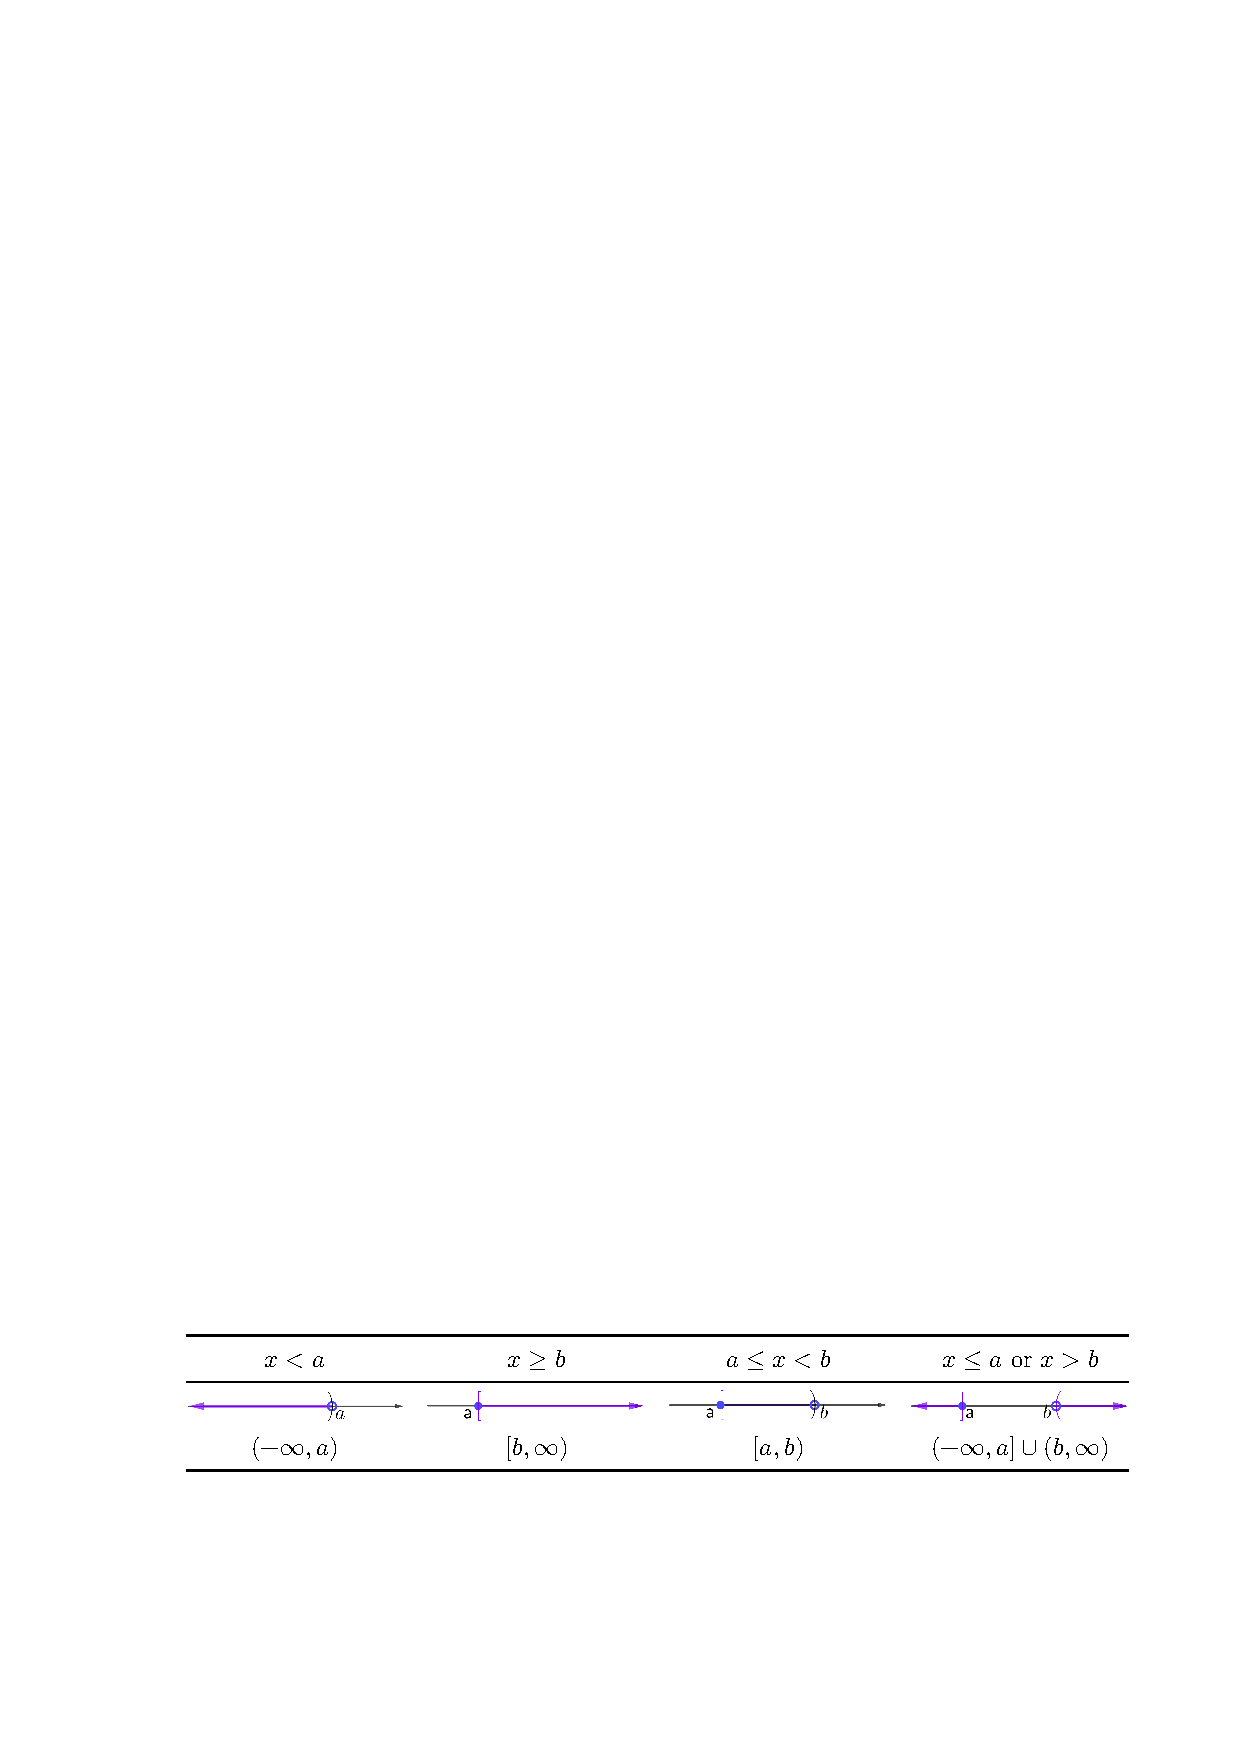
\includegraphics[width=0.8\linewidth]{figs/linear-inequalities.pdf}
  }
\end{fullwidth}
% 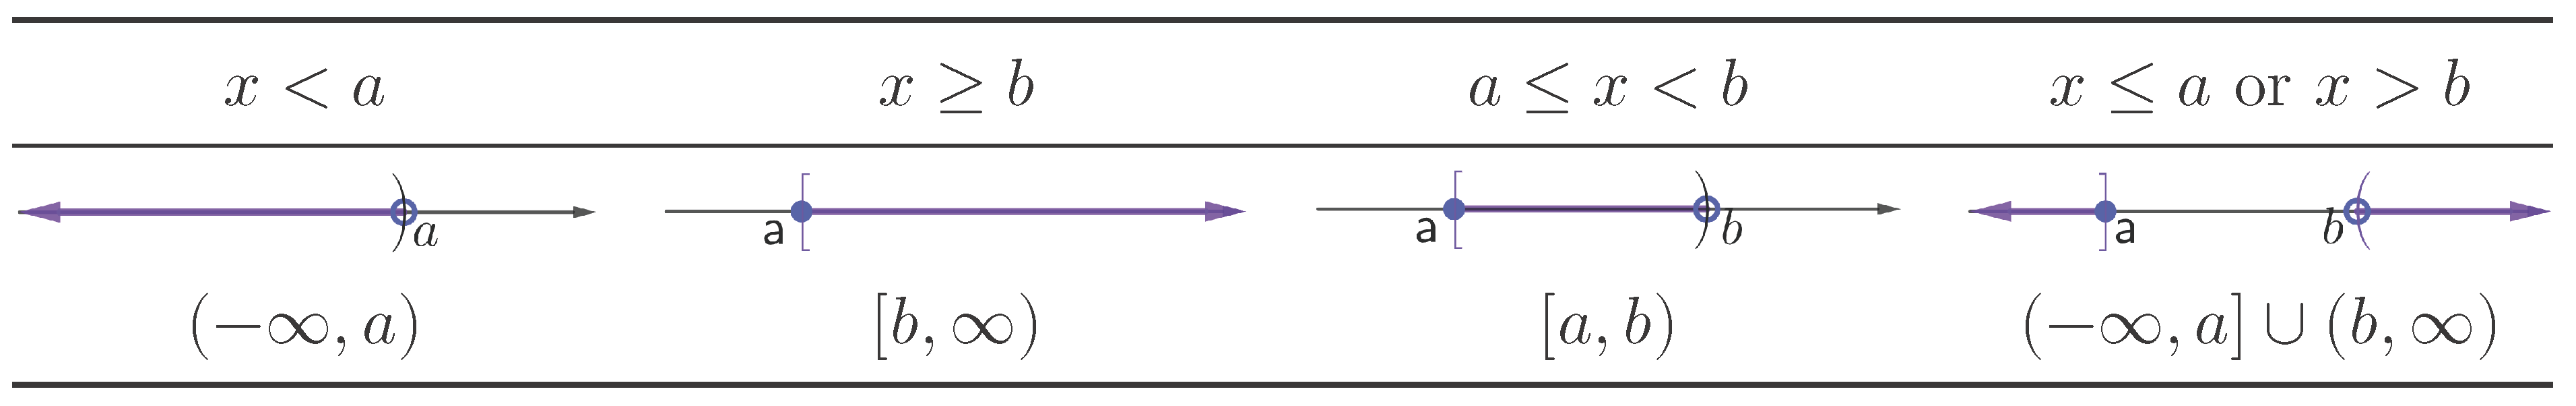
\includegraphics{figs/linear-inequalities.png}

\begin{example}

Solve the linear inequality \[
2x+4>0.
\]

\end{example}
\vspace*{6\baselineskip}

\begin{example}

Solve the linear inequality \[
-3x-4<2.
\]

\end{example}
\vspace*{6\baselineskip}

\begin{example}

Solve the compound linear inequality \[
x+2<3\quad \text{and}\quad -2x-3<1.
\]

\end{example}
\vspace*{6\baselineskip}

\begin{example}

Solve the compound linear inequality\\
\[
-x+4>2 \quad \text{or} \quad 2x-5\geq -3.
\]

\end{example}
\vspace*{6\baselineskip}

\begin{example}

Solve the compound linear inequality \[
-4\leq\dfrac{2x-4}{3}<2.
\]

\end{example}
\vspace*{6\baselineskip}

\begin{example}

Solve the compound linear inequality \[
-1\leq \dfrac{-3x+4}{2}<3.
\]

\end{example}
\vspace*{6\baselineskip}

\begin{example}

Suppose that \(-1\le x < 2\). Find the range of \(5-3x\). Write your
answer in interval notation.

\end{example}
\vspace*{6\baselineskip}

\subsection{Practice}

\begin{exercise}

Solve the linear inequality. \textbf{Write your answer in interval
notation.}

\begin{enumerate}
\item
  \(3x + 7 \leq 1\)
\item
  \(2x-3>1\)
\end{enumerate}

\end{exercise}

\begin{exercise}

Solve the linear inequality. \textbf{Write your answer in interval
notation.}

\begin{enumerate}
\item
  \(4x + 7 > 2x-3\)
\item
  \(3-2x \le x-6\)
\end{enumerate}

\end{exercise}

\begin{exercise}

Solve the compound linear inequality. \textbf{Write your answer in
interval notation.}

\begin{enumerate}
\item
  \(3x+2>-1 ~\text{and}~ 2x-7\leq 1\)
\item
  \(4x -7< 5 ~\text{and}~ 5x-2\geq 3\)
\end{enumerate}

\end{exercise}

\begin{exercise}

Solve the compound linear inequality. \textbf{Write your answer in
interval notation.}

\begin{enumerate}
\item
  \(-4\leq 3x+5<11\)
\item
  \(7\geq 2x-3\geq -7\)
\end{enumerate}

\end{exercise}

\begin{exercise}

Solve the compound linear inequality. \textbf{Write your answer in
interval notation.}

\begin{enumerate}
\item
  \(3x-5>-2 ~\text{or}~ 10-2x\leq 4\)
\item
  \(2x + 7<5 ~\text{or}~ 3x-8\geq x-2\)
\end{enumerate}

\end{exercise}

\begin{exercise}

Solve the compound linear inequality. \textbf{Write your answer in
interval notation.}

\begin{enumerate}
\item
  \(-2\leq \dfrac{2x-5}{3}<3\)
\item
  \(-1< \dfrac{3x+7}{2}\leq 4\)
\end{enumerate}

\end{exercise}

\begin{exercise}

Solve the linear inequality. \textbf{Write your answer in interval
notation.} \[
\frac13x+1<\frac12(2x-3)-1
\]

\end{exercise}

\vspace*{6\baselineskip}

\begin{exercise}

Solve the compound linear inequality. \textbf{Write your answer in
interval notation.} \[
0\le \frac25-\frac{x+1}{3}< 1
\]

\end{exercise}

\vspace*{6\baselineskip}

\begin{exercise}

Suppose \(0< x \le 1\). Find the range of \(-2x+1\). \textbf{Write your
answer in interval notation.}

\end{exercise}

\vspace*{6\baselineskip}

\begin{exercise}

Suppose that \(x+2y=1\) and \(1\leq x< 3\). Find the range of \(y\).
\textbf{Write your answer in interval notation.}

\end{exercise}
\vspace*{6\baselineskip}

\begin{exercise}

A toy store has a promotion ``Buy one get the second one half price'' on
a certain popular toy. The sale price of the toy is \$20 each. Suppose
the store makes more profit when you buy two. What do you think the
store's purchasing price of the toy is?

\end{exercise}


